\chapter{Literature review}
\label{ch:literature-review}

This chapter establishes the theoretical and empirical foundation and background for integrating a resource-augmented AI assistant into Sovelia Core PLM. The review begins by examining the fundamental characteristics of Product Lifecycle Management systems and the role of AI assistants in data-intensive workflows, establishing why a human-in-the-loop considerable approach for enterprise PLM environments (\autoref{sec:plm-systems-and-ai-assistants}). After this, the overall architecture and principles of Retrieval-Augmented Generation (RAG) systems is explained briefly, focusing on how the combination of parametric and non-parametric memory addresses key limitations of purely parametric models in knowledge-intensive tasks (\autoref{sec:resource-augmented-ai-systems}).

The core of this review examines five recent case studies of RAG-based systems deployed in technical documentation and manufacturing contexts (\autoref{sec:case-studies-on-similar-integrations}): Heredia Álvaro and Barreda's ceramic tile manufacturing quality control system, Shejuti et al.'s technical documentation chatbot, Knollmeyer et al.'s manufacturing documentation system with knowledge graph enhancement, Wan et al.'s hybrid KG-vector RAG for smart manufacturing, and Wang et al.'s comprehensive framework for AI in PLM. These studies reveal both common success factors, particularly in domain-specific adaptation, and persistent challenges. The contexts of these studies are comparable to those of typical PLM system users, who are predominantly in the manufacturing industry \parencite{stark_product_2015}. By synthesizing lessons from these deployments, this review identifies key design considerations and risk factors to inform the architecture and implementation strategy of the AI assistant for Sovelia Core, especially given the challenges faced by companies in the manufacturing industry.

\section{Overview of PLM systems and AI assistants}
\label{sec:plm-systems-and-ai-assistants}

Product Lifecycle Management (PLM) systems are integral to managing the entire lifecycle of a product from inception, through engineering design and manufacturing, to service and disposal. They provide a centralized repository for all product-related information, facilitating collaboration among different departments and stakeholders \parencite{stark_product_2015}. In PLM systems generally the lifecycle states of product include: imagine, define, realise, support/use and retire/dispose \parencite{stark_product_2015-1}. All these separate stages generate data (including documentation) that needs to be managed effectively. The purpose of PLM system is to centralize all this data and provide users with access to the right information at the right time.

AI assistants, in the context of data-intensive workflows, can be defined as \textit{semi-automatic interactive tools} that guide analysts through specific tasks by recommending suitable transformations or actions that respect constraints obtained through interaction with the analyst \parencite{petricek_ai_2023}. Analysts in this context mean the human utilizing the AI assistant. Unlike fully automatic systems that attempt to solve problems without human intervention, or purely manual tools that require complete human control, AI assistants implement an iterative interaction pattern where the system makes an initial recommendation, the user can provide feedback through structured constraints or selections, and the system refines its recommendations accordingly. This human-in-the-loop approach combines the scalability and automation of machine learning with critical human insight, making it particularly suitable for tasks where edge cases and domain-specific knowledge are crucial \parencite{petricek_ai_2023}. In this thesis, the aim is to develop an AI assistant that can be integrated into PLM system to enhance user experience by providing context-aware support, streamlining routine data wrangling tasks, and improving access to information while maintaining human oversight and control. The AI assistant is meant to provide users with answers based on the documentation stored within the PLM system's database. However, the AI assistant in the context of this thesis is not fully automatic, as the users still have control over the final decisions and actions taken based on the AI assistant's recommendations. The purpose of the AI assistant is to inform and help with decision-making, rather than replacing human judgment entirely.

\section{Resource-augmented AI systems}
\label{sec:resource-augmented-ai-systems}

Resource-augmented AI systems, also known as \emph{retrieval-augmented generation} (RAG) systems, represent a paradigm shift in how artificial intelligence systems access and utilize knowledge. Unlike purely parametric models that store all knowledge implicitly within their parameters, resource-augmented systems combine parametric memory (the weights of a neural network) with non-parametric memory (external knowledge sources such as databases, document collections, or knowledge graphs) \parencite{lewis_retrieval-augmented_2021}. This hybrid architecture addresses several fundamental limitations of parametric-only models: the inability to easily update or revise stored knowledge, difficulty in providing provenance for predictions, and the tendency to generate hallucinated or factually incorrect content \parencite{lewis_retrieval-augmented_2021}. In simplified terms, RAG systems can be viewed as AI systems that "look up" relevant information from an external source before generating a response, rather than relying solely on learned patterns from training data and thus enabling more accurate, up-to-date, and contextually relevant outputs. This will result in less hallucinations compared to standard large language models (LLMs) \parencite{lewis_retrieval-augmented_2021}.

\begin{figure}[htbp]
    \centering
    \small{\resizebox{\textwidth}{!}{% generated by Plantuml 1.2025.9       
\definecolor{plantucolor0000}{RGB}{0,0,0}
\definecolor{plantucolor0001}{RGB}{255,255,255}
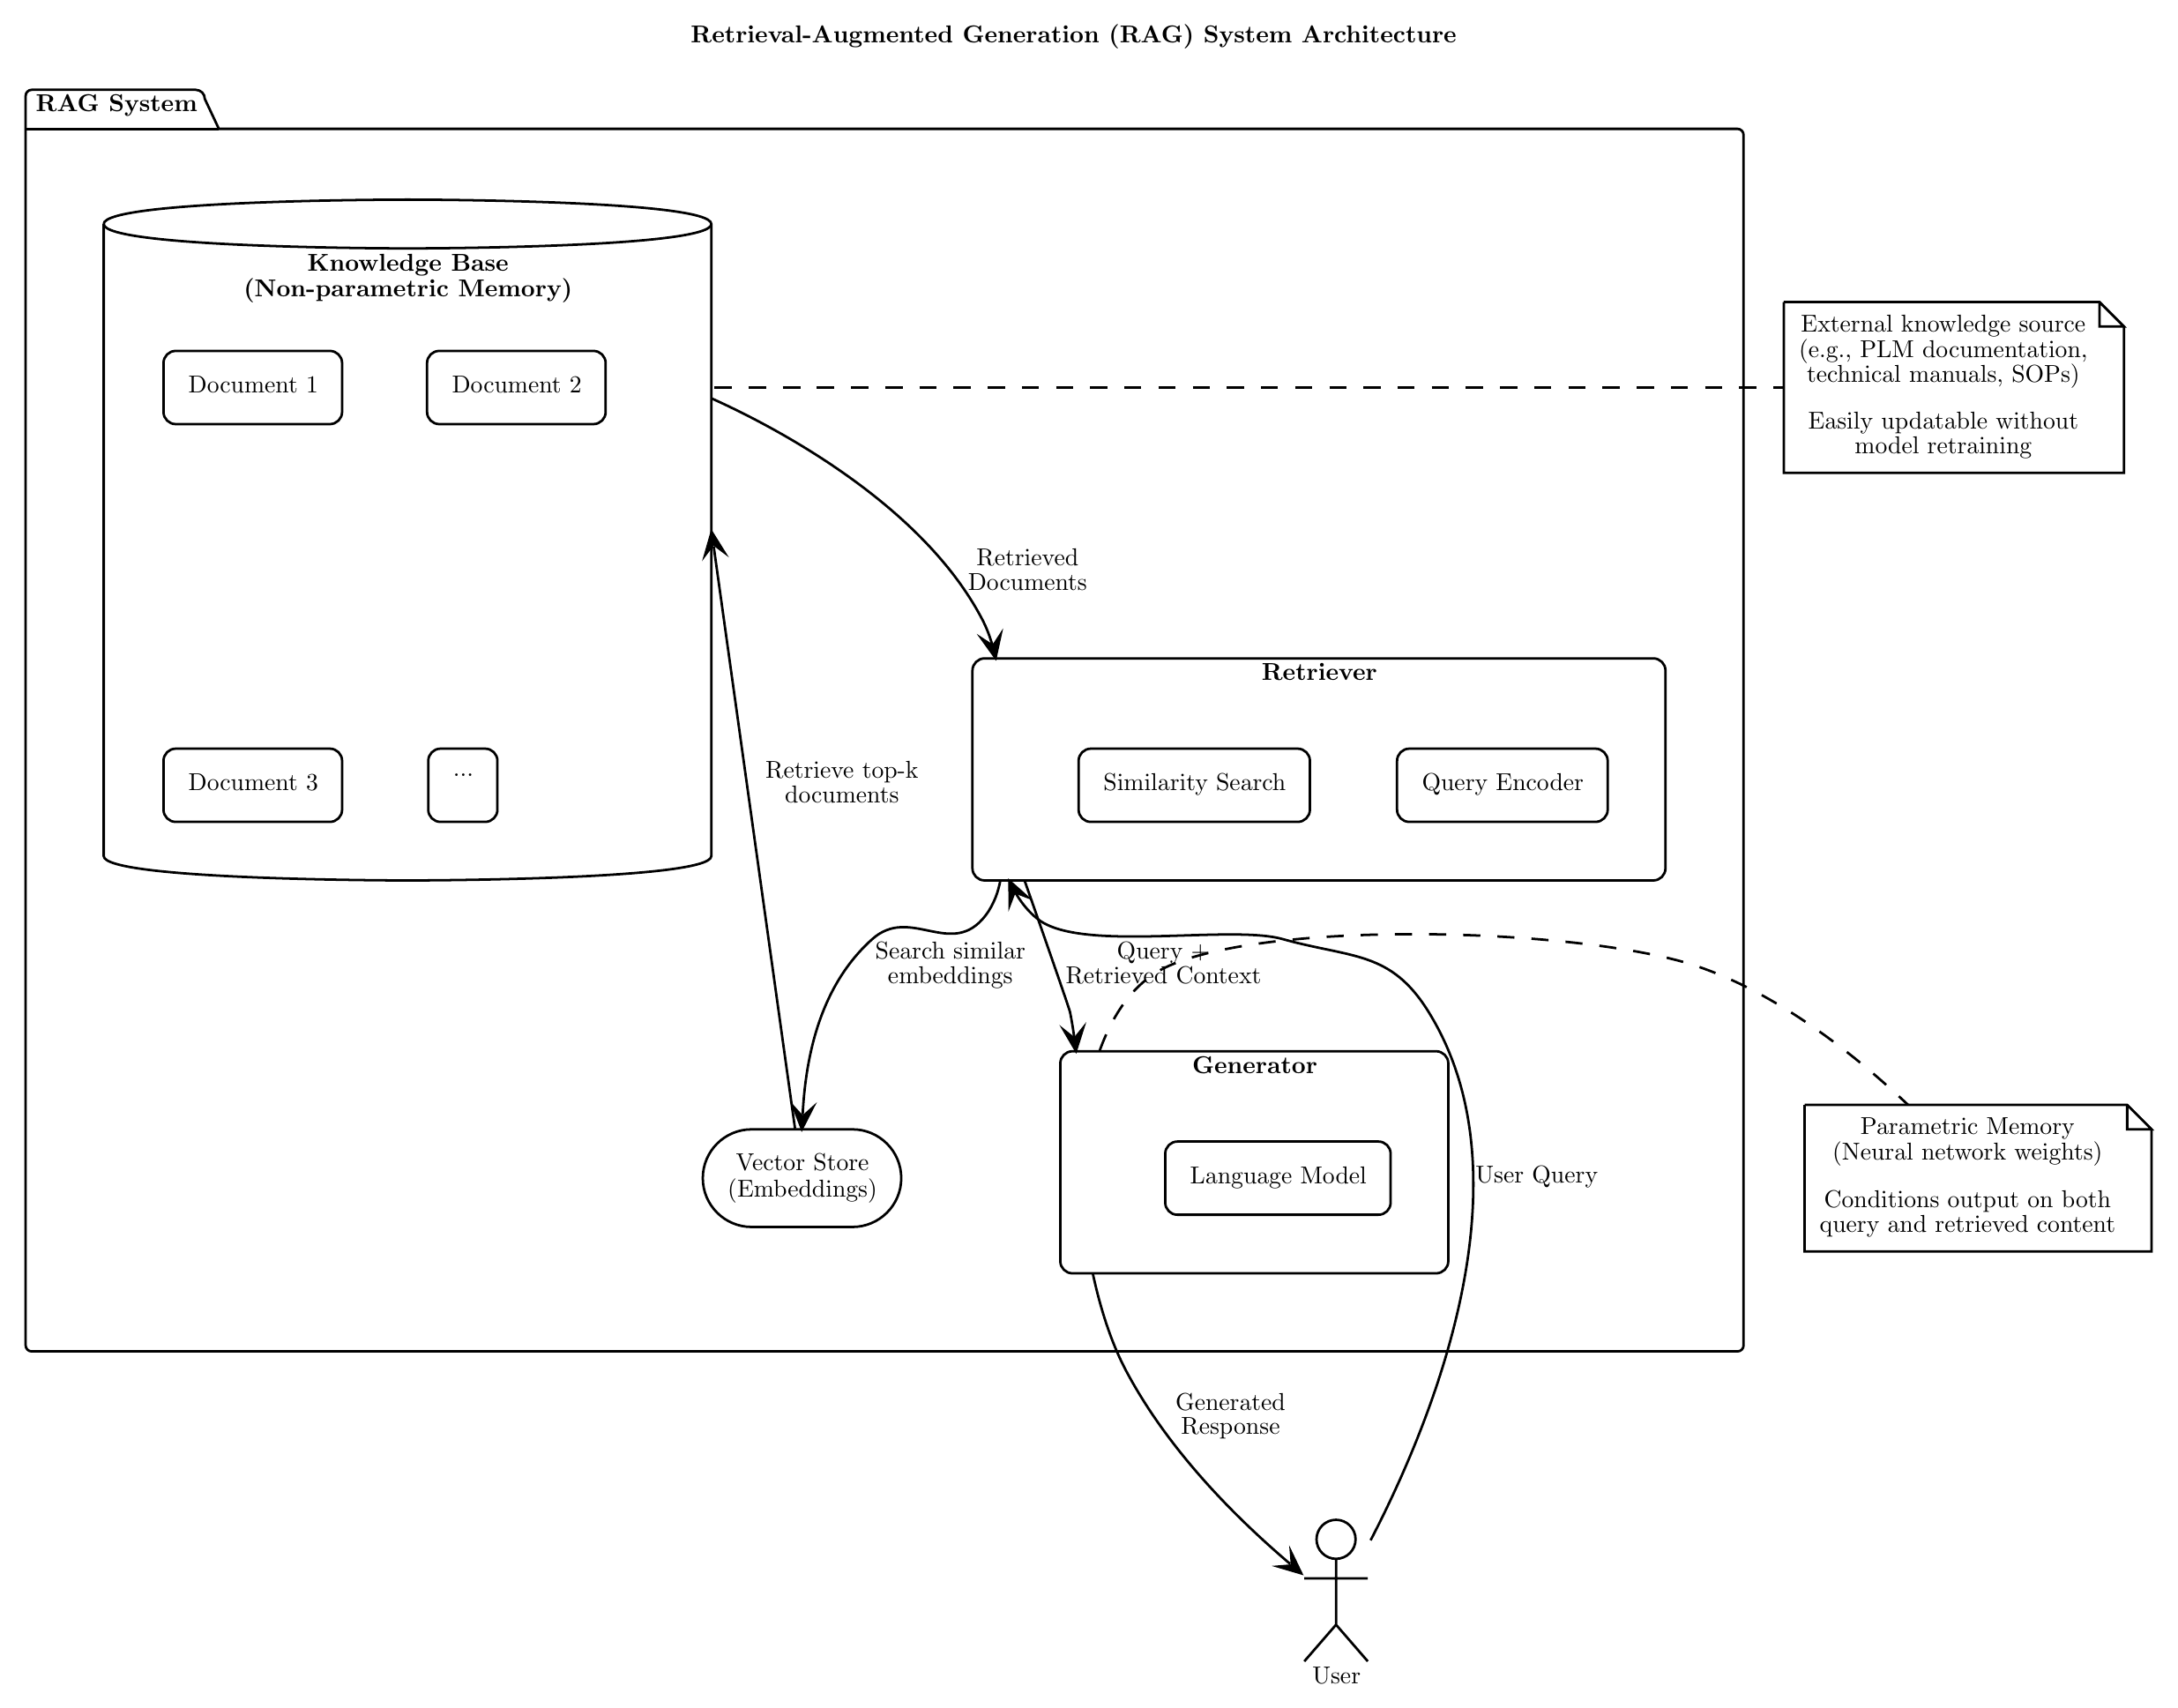
\begin{tikzpicture}[yscale=-1
,pstyle0/.style={color=black,fill=white,line width=1.0pt}
,pstyle1/.style={color=black,line width=1.0pt}
,pstyle2/.style={color=black,fill=black,line width=1.0pt}
,pstyle3/.style={color=black,line width=1.0pt,dash pattern=on 7.0pt off 7.0pt}
]
\node at (283.395pt,15pt)[below right,color=black,inner sep=0]{\textbf{Retrieval-Augmented Generation (RAG) System Architecture}};
\draw[pstyle0] (13.5pt,42pt) -- (80.69pt,42pt) arc(270:360:3.75pt)  -- (90.19pt,58pt) -- (712.5pt,58pt) arc(270:360:2.5pt)  -- (715pt,556.5pt) arc(0:90:2.5pt)  -- (13.5pt,559pt) arc(90:180:2.5pt)  -- (11pt,44.5pt) arc(180:270:2.5pt) ;
\draw[pstyle1] (11pt,58pt) -- (90.19pt,58pt);
\node at (15pt,44pt)[below right,color=black,inner sep=0]{\textbf{RAG System}};
\draw[pstyle0] (399pt,280pt) arc (180:270:5pt) -- (404pt,275pt) -- (678pt,275pt) arc (270:360:5pt) -- (683pt,280pt) -- (683pt,361pt) arc (0:90:5pt) -- (678pt,366pt) -- (404pt,366pt) arc (90:180:5pt) -- (399pt,361pt) -- cycle;
\node at (517.335pt,277pt)[below right,color=black,inner sep=0]{\textbf{Retriever}};
\draw[pstyle0] (435pt,441pt) arc (180:270:5pt) -- (440pt,436pt) -- (589pt,436pt) arc (270:360:5pt) -- (594pt,441pt) -- (594pt,522pt) arc (0:90:5pt) -- (589pt,527pt) -- (440pt,527pt) arc (90:180:5pt) -- (435pt,522pt) -- cycle;
\node at (488.87pt,438pt)[below right,color=black,inner sep=0]{\textbf{Generator}};
\draw[pstyle0] (43pt,97pt) ..controls (43pt,87pt) and (167.5pt,87pt) .. (167.5pt,87pt) ..controls (167.5pt,87pt) and (292pt,87pt) .. (292pt,97pt) -- (292pt,356pt) ..controls (292pt,366pt) and (167.5pt,366pt) .. (167.5pt,366pt) ..controls (167.5pt,366pt) and (43pt,366pt) .. (43pt,356pt) -- (43pt,97pt);
\draw[pstyle1] (43pt,97pt) ..controls (43pt,107pt) and (167.5pt,107pt) .. (167.5pt,107pt) ..controls (167.5pt,107pt) and (292pt,107pt) .. (292pt,97pt);
\node at (126.29pt,109pt)[below right,color=black,inner sep=0]{\textbf{Knowledge Base}};
\node at (100.13pt,119pt)[below right,color=black,inner sep=0]{\textbf{(Non-parametric Memory)}};
\draw[pstyle0] (288.5pt,488pt) arc (180:270:20pt) -- (308.5pt,468pt) -- (349.82pt,468pt) arc (270:360:20pt) -- (369.82pt,488pt) -- (369.82pt,488pt) arc (0:90:20pt) -- (349.82pt,508pt) -- (308.5pt,508pt) arc (90:180:20pt) -- (288.5pt,488pt) -- cycle;
\node at (301.91pt,478pt)[below right,color=black,inner sep=0]{Vector Store};
\node at (298.5pt,488pt)[below right,color=black,inner sep=0]{(Embeddings)};
\draw[pstyle0] (573pt,317pt) arc (180:270:5pt) -- (578pt,312pt) -- (654.32pt,312pt) arc (270:360:5pt) -- (659.32pt,317pt) -- (659.32pt,337pt) arc (0:90:5pt) -- (654.32pt,342pt) -- (578pt,342pt) arc (90:180:5pt) -- (573pt,337pt) -- cycle;
\node at (583pt,322pt)[below right,color=black,inner sep=0]{Query Encoder};
\draw[pstyle0] (442.5pt,317pt) arc (180:270:5pt) -- (447.5pt,312pt) -- (532.29pt,312pt) arc (270:360:5pt) -- (537.29pt,317pt) -- (537.29pt,337pt) arc (0:90:5pt) -- (532.29pt,342pt) -- (447.5pt,342pt) arc (90:180:5pt) -- (442.5pt,337pt) -- cycle;
\node at (452.5pt,322pt)[below right,color=black,inner sep=0]{Similarity Search};
\draw[pstyle0] (478pt,478pt) arc (180:270:5pt) -- (483pt,473pt) -- (565.37pt,473pt) arc (270:360:5pt) -- (570.37pt,478pt) -- (570.37pt,498pt) arc (0:90:5pt) -- (565.37pt,503pt) -- (483pt,503pt) arc (90:180:5pt) -- (478pt,498pt) -- cycle;
\node at (488pt,483pt)[below right,color=black,inner sep=0]{Language Model};
\draw[pstyle0] (67.5pt,154pt) arc (180:270:5pt) -- (72.5pt,149pt) -- (135.69pt,149pt) arc (270:360:5pt) -- (140.69pt,154pt) -- (140.69pt,174pt) arc (0:90:5pt) -- (135.69pt,179pt) -- (72.5pt,179pt) arc (90:180:5pt) -- (67.5pt,174pt) -- cycle;
\node at (77.5pt,159pt)[below right,color=black,inner sep=0]{Document 1};
\draw[pstyle0] (175.5pt,154pt) arc (180:270:5pt) -- (180.5pt,149pt) -- (243.69pt,149pt) arc (270:360:5pt) -- (248.69pt,154pt) -- (248.69pt,174pt) arc (0:90:5pt) -- (243.69pt,179pt) -- (180.5pt,179pt) arc (90:180:5pt) -- (175.5pt,174pt) -- cycle;
\node at (185.5pt,159pt)[below right,color=black,inner sep=0]{Document 2};
\draw[pstyle0] (67.5pt,317pt) arc (180:270:5pt) -- (72.5pt,312pt) -- (135.69pt,312pt) arc (270:360:5pt) -- (140.69pt,317pt) -- (140.69pt,337pt) arc (0:90:5pt) -- (135.69pt,342pt) -- (72.5pt,342pt) arc (90:180:5pt) -- (67.5pt,337pt) -- cycle;
\node at (77.5pt,322pt)[below right,color=black,inner sep=0]{Document 3};
\draw[pstyle0] (176pt,317pt) arc (180:270:5pt) -- (181pt,312pt) -- (199.34pt,312pt) arc (270:360:5pt) -- (204.34pt,317pt) -- (204.34pt,337pt) arc (0:90:5pt) -- (199.34pt,342pt) -- (181pt,342pt) arc (90:180:5pt) -- (176pt,337pt) -- cycle;
\node at (186pt,322pt)[below right,color=black,inner sep=0]{...};
\draw[pstyle0] (548pt,636pt) ellipse (8pt and 8pt);
\draw[pstyle1] (548pt,644pt) -- (548pt,671pt)(535pt,652pt) -- (561pt,652pt)(548pt,671pt) -- (535pt,686pt)(548pt,671pt) -- (561pt,686pt);
\node at (538.1pt,688pt)[below right,color=black,inner sep=0]{User};
\draw[pstyle0] (731.5pt,129pt) -- (731.5pt,199pt) -- (870.85pt,199pt) -- (870.85pt,139pt) -- (860.85pt,129pt) -- (731.5pt,129pt);
\draw[pstyle0] (860.85pt,129pt) -- (860.85pt,139pt) -- (870.85pt,139pt) -- (860.85pt,129pt);
\node at (738.355pt,134pt)[below right,color=black,inner sep=0]{External knowledge source};
\node at (737.5pt,144pt)[below right,color=black,inner sep=0]{(e.g., PLM documentation,};
\node at (740.715pt,154pt)[below right,color=black,inner sep=0]{technical manuals, SOPs)};
\node at (795.01pt,164pt)[below right,color=black,inner sep=0]{~};
\node at (741.285pt,174pt)[below right,color=black,inner sep=0]{Easily updatable without};
\node at (760.39pt,184pt)[below right,color=black,inner sep=0]{model retraining};
\draw[pstyle0] (740pt,458pt) -- (740pt,518pt) -- (882.2pt,518pt) -- (882.2pt,468pt) -- (872.2pt,458pt) -- (740pt,458pt);
\draw[pstyle0] (872.2pt,458pt) -- (872.2pt,468pt) -- (882.2pt,468pt) -- (872.2pt,458pt);
\node at (762.74pt,463pt)[below right,color=black,inner sep=0]{Parametric Memory};
\node at (751.27pt,473pt)[below right,color=black,inner sep=0]{(Neural network weights)};
\node at (804.935pt,483pt)[below right,color=black,inner sep=0]{~};
\node at (747.805pt,493pt)[below right,color=black,inner sep=0]{Conditions output on both};
\node at (746pt,503pt)[below right,color=black,inner sep=0]{query and retrieved content};
\draw[pstyle1] (562.16pt,636.4pt) ..controls (586.27pt,589.98pt) and (628.73pt,489.14pt) .. (586pt,420pt) ..controls (570.33pt,394.64pt) and (554.72pt,398pt) .. (526pt,390pt) ..controls (504.52pt,384.02pt) and (443.66pt,395.6pt) .. (426pt,382pt) ..controls (421.1175pt,378.24pt) and (417.4856pt,373.1338pt) .. (414.785pt,367.5539pt) ..controls (414.6162pt,367.2052pt) and (414.4511pt,366.8546pt) .. (414.2895pt,366.5023pt) ..controls (414.2491pt,366.4143pt) and (416.6833pt,371.7921pt) .. (416.6434pt,371.7039pt);
\draw[pstyle2] (414.1689pt,366.2379pt) -- (414.2366pt,376.0865pt) -- (416.231pt,370.7929pt) -- (421.5246pt,372.7872pt) -- (414.1689pt,366.2379pt) -- cycle;
\node at (605pt,483pt)[below right,color=black,inner sep=0]{User Query};
\draw[pstyle1] (410.4238pt,366.0457pt) ..controls (410.3895pt,366.2243pt) and (410.3542pt,366.4026pt) .. (410.3178pt,366.5806pt) ..controls (409.1531pt,372.2775pt) and (406.905pt,377.675pt) .. (403pt,382pt) ..controls (389.39pt,397.08pt) and (373.16pt,376.48pt) .. (358pt,390pt) ..controls (335.83pt,409.77pt) and (330.6147pt,439.7188pt) .. (329.4147pt,461.8588pt);
\draw[pstyle2] (329.09pt,467.85pt) -- (333.5712pt,459.0797pt) -- (329.3606pt,462.8573pt) -- (325.583pt,458.6467pt) -- (329.09pt,467.85pt) -- cycle;
\node at (359pt,391pt)[below right,color=black,inner sep=0]{Search similar};
\node at (364.165pt,401pt)[below right,color=black,inner sep=0]{embeddings};
\draw[pstyle1] (326.29pt,467.63pt) ..controls (321.475pt,433.17pt) and (311.0525pt,358.58pt) .. (301.76pt,292.0788pt) ..controls (299.4369pt,275.4534pt) and (297.1844pt,259.3337pt) .. (295.1078pt,244.4729pt) ..controls (294.0695pt,237.0425pt) and (293.9055pt,235.8691pt) .. (292.9683pt,229.1623pt);
\draw[pstyle2] (292.138pt,223.2201pt) -- (289.422pt,232.687pt) -- (292.8299pt,228.172pt) -- (297.345pt,231.5799pt) -- (292.138pt,223.2201pt) -- cycle;
\node at (314pt,317pt)[below right,color=black,inner sep=0]{Retrieve top-k};
\node at (321.97pt,327pt)[below right,color=black,inner sep=0]{documents};
\draw[pstyle1] (292.0848pt,168.4581pt) ..controls (292.5082pt,168.6482pt) and (292.9461pt,168.846pt) .. (293.3979pt,169.0515pt) ..controls (295.2052pt,169.8734pt) and (297.2355pt,170.8183pt) .. (299.455pt,171.8842pt) ..controls (308.3331pt,176.1478pt) and (320.24pt,182.3469pt) .. (333.0225pt,190.3513pt) ..controls (358.5875pt,206.36pt) and (387.655pt,229.59pt) .. (403pt,259pt) ..controls (404.6713pt,262.2025pt) and (405.9964pt,265.6119pt) .. (407.0348pt,269.1311pt) ..controls (407.554pt,270.8906pt) and (408.0015pt,272.6777pt) .. (408.3847pt,274.48pt) ..controls (408.4086pt,274.5927pt) and (407.2107pt,268.8311pt) .. (407.2342pt,268.9438pt);
\draw[pstyle2] (408.4558pt,274.8182pt) -- (410.5396pt,265.1923pt) -- (407.4378pt,269.9229pt) -- (402.7071pt,266.8211pt) -- (408.4558pt,274.8182pt) -- cycle;
\node at (400.485pt,230pt)[below right,color=black,inner sep=0]{Retrieved};
\node at (397pt,240pt)[below right,color=black,inner sep=0]{Documents};
\draw[pstyle1] (420.439pt,366.2539pt) ..controls (420.4993pt,366.426pt) and (420.5597pt,366.5983pt) .. (420.6201pt,366.7708pt) ..controls (420.7409pt,367.1156pt) and (420.8619pt,367.4611pt) .. (420.9831pt,367.807pt) ..controls (421.2255pt,368.4988pt) and (421.4684pt,369.1925pt) .. (421.7118pt,369.8875pt) ..controls (422.1985pt,371.2775pt) and (422.6869pt,372.6725pt) .. (423.175pt,374.0675pt) ..controls (430.985pt,396.3875pt) and (438.74pt,418.695pt) .. (439pt,420pt) ..controls (439.7075pt,423.5425pt) and (440.3023pt,427.2095pt) .. (440.8014pt,430.919pt) ..controls (440.9262pt,431.8463pt) and (441.045pt,432.7764pt) .. (441.1581pt,433.7077pt) ..controls (441.2146pt,434.1734pt) and (441.2697pt,434.6395pt) .. (441.3234pt,435.1057pt) ..controls (441.3503pt,435.3388pt) and (440.7079pt,429.6094pt) .. (440.734pt,429.8425pt);
\draw[pstyle2] (441.403pt,435.8051pt) -- (444.3746pt,426.4153pt) -- (440.8455pt,430.8363pt) -- (436.4245pt,427.3072pt) -- (441.403pt,435.8051pt) -- cycle;
\node at (458.035pt,391pt)[below right,color=black,inner sep=0]{Query +};
\node at (437pt,401.1pt)[below right,color=black,inner sep=0]{Retrieved Context};
\draw[pstyle1] (448.3779pt,527.354pt) ..controls (448.4338pt,527.6107pt) and (448.4902pt,527.8679pt) .. (448.5472pt,528.1255pt) ..controls (448.6612pt,528.6409pt) and (448.7775pt,529.1581pt) .. (448.896pt,529.6771pt) ..controls (449.8445pt,533.8285pt) and (450.9404pt,538.0877pt) .. (452.2055pt,542.3453pt) ..controls (454.7356pt,550.8606pt) and (457.9425pt,559.37pt) .. (462pt,567pt) ..controls (480.43pt,601.67pt) and (509.9206pt,629.6815pt) .. (529.1806pt,646.0715pt);
\draw[pstyle2] (533.75pt,649.96pt) -- (529.4882pt,641.081pt) -- (529.9422pt,646.7196pt) -- (524.3035pt,647.1735pt) -- (533.75pt,649.96pt) -- cycle;
\node at (482pt,576pt)[below right,color=black,inner sep=0]{Generated};
\node at (484.29pt,586pt)[below right,color=black,inner sep=0]{Response};
\draw[pstyle3] (293.2287pt,164pt) ..controls (293.8106pt,164pt) and (294.3925pt,164pt) .. (294.9744pt,164pt) ..controls (296.1383pt,164pt) and (297.3021pt,164pt) .. (298.4659pt,164pt) ..controls (303.1212pt,164pt) and (307.7765pt,164pt) .. (312.4318pt,164pt) ..controls (321.7423pt,164pt) and (331.0528pt,164pt) .. (340.3633pt,164pt) ..controls (358.9843pt,164pt) and (377.6051pt,164pt) .. (396.2258pt,164pt) ..controls (433.4672pt,164pt) and (470.7081pt,164pt) .. (507.9488pt,164pt) ..controls (582.43pt,164pt) and (656.91pt,164pt) .. (731.39pt,164pt);
\draw[pstyle3] (451.1901pt,435.6097pt) ..controls (451.4022pt,435.0226pt) and (451.6198pt,434.437pt) .. (451.8429pt,433.8535pt) ..controls (453.628pt,429.1855pt) and (455.7711pt,424.6478pt) .. (458.3434pt,420.4494pt) ..controls (463.4881pt,412.0525pt) and (470.35pt,405.0125pt) .. (479.5pt,401pt) ..controls (523.46pt,381.72pt) and (649.98pt,385.77pt) .. (695.5pt,401pt) ..controls (729.07pt,412.23pt) and (760.7pt,437.48pt) .. (782.34pt,457.9pt);
\end{tikzpicture}
}}
    \caption{Retrieval-Augmented Generation (RAG) system architecture}
    \label{fig:rag-architecture}
\end{figure}

In a typical RAG architecture, the system consists of two main components: a \emph{retriever} that identifies relevant documents or passages from an external knowledge source given an input query, and a \emph{generator} that produces outputs conditioned on both the input and the retrieved content \parencite{lewis_retrieval-augmented_2021}. The retriever typically employs dense passage retrieval methods using bi-encoder architectures that compute semantic similarity between queries and documents in a shared embedding space, while the generator is commonly implemented as a pre-trained sequence-to-sequence transformer model. Crucially, these components can be trained end-to-end, allowing the retrieval mechanism to learn what information is relevant for the downstream task without requiring explicit retrieval supervision. \autoref{fig:rag-architecture} illustrates this architecture, showing how user queries flow through the retriever to access the knowledge base, and how retrieved context is combined with the query in the generator to produce responses.

\textcite{lewis_retrieval-augmented_2021} have highlighted that the advantages of resource-augmented systems are particularly pronounced in knowledge-intensive tasks. There are tasks that humans could not reasonably perform without access to external knowledge sources. By maintaining knowledge in an explicit, inspectable, and easily updatable non-parametric form, these systems enable dynamic knowledge updates by simply replacing or modifying the external knowledge source (a process sometimes called "index hot-swapping") without requiring costly model retraining and allowing for customizability for different needs. Additionally, the retrieved documents allow users to understand what information informed the system's response. In the context of PLM systems, this architecture is particularly well-suited for handling the extensive, evolving documentation ecosystem that characterizes enterprise software deployments. The customizable nature of RAG systems allow for tailoring the knowledge and thus the responses to the specific configurations and processes of different organizations using the PLM system.

\section{Case studies on similar integrations}
\label{sec:case-studies-on-similar-integrations}

Several recent implementations of RAG-based systems for technical documentation and manufacturing environments provide valuable insights for the design and development of an AI assistant for Sovelia Core, the main topic of this thesis. This section examines four representative case studies that demonstrate both the feasibility and challenges of integrating RAG technology into similarly complex technical domains.

\subsection*{Manufacturing quality control: Heredia Álvaro and Barreda's ceramic tile RAG system}

Heredia Álvaro and Barreda (2025) developed an advanced RAG system for manufacturing quality control in the ceramic tile industry \parencite{heredia_alvaro_advanced_2025}, addressing challenges comparable to those in PLM environments. Notably, as any companies in the manufacturing industry, ceramic tile manufacturers can be seen as potential PLM system users and thus, face similar issues with knowledge silos in technical documentation. In the study there are many similar characteristics mentioned: extensive technical documentation (defect handbooks, process articles), multiple specialized stages requiring expert knowledge (pressing, drying, enameling, firing, finishing), and the need for rapid procedural access for defect diagnosis and root cause analysis by users with varying expertise levels.

The system architecture detailed in the study employed a straightforward RAG implementation using OpenAI's text-embedding-3-large model for document indexing, with a pre-processing pipeline that structured 221 samples of ceramic defect information (defect type, identification methods, causes, solutions, origin areas). Documents were processed through validation mechanisms, with short documents fed directly to the LLM and longer documents first fragmented and stored in a Chroma vector store. Notably, Heredia Álvaro and Barreda implemented a two-stage retrieval approach: initial retrieval using a bi-encoder with Euclidean distance similarity, followed by post-retrieval reranking using a cross-encoder (sentence transformers ms-frame-MiniLM-L-6-v2) to prioritize the most relevant information samples. This combination addresses the computational trade-offs between efficiency (bi-encoder) and accuracy (cross-encoder). The generator itself used OpenAI's gpt-3.5-turbo-instruct model with customized prompts to make sure that responses prioritized external knowledge over the model's parametric memory. \parencite{heredia_alvaro_advanced_2025}

The system demonstrated practical effectiveness after the evaluation using both retrieval and generation metrics. The retrieval phase achieved 92.68\% Jaccard similarity and 85.81\% F1-score with optimal hyperparameters (k=7 retrieved samples, mean relevance score threshold), indicating high precision in identifying relevant context. The generation phase evaluation using ROUGE-L metrics yielded a mean score of 0.6108 (standard deviation 0.1371), significantly outperforming random baselines (mean 0.2300). Qualitative comparison against GPT-4 without domain adaptation demonstrated the RAG system's superiority in providing accurate, domain-specific answers. For example, when queried about carbon particles in ceramic tiles, the RAG system correctly identified the defect as impurities in raw materials and recommended weathering clays or finer sieving, whereas GPT-4 incorrectly attributed the issue to general fouling and cleaning problems. The system operates at low computational cost (approximately \$0.0012 per query) and achieved practical deployment for use cases including customer claim resolution, non-conformities reporting, and continuous improvement actions. \parencite{heredia_alvaro_advanced_2025}

For the Sovelia Core PLM integration, Heredia Álvaro and Barreda's work provides directly applicable insights aligned with this thesis's scope. Their implementation represents a pragmatic approach prioritizing foundational RAG capabilities over advanced techniques. The architecture demonstrates several design principles relevant to enterprise PLM deployment: (1) careful pre-processing and post-processing to optimize retrieval quality without requiring model fine-tuning, (2) systematic hyperparameter optimization through evaluation metrics, (3) structured knowledge representation (defect types, causes, solutions) that is similar to PLM documentation patterns, and (4) explicit validation mechanisms to ensure query relevance. The study's emphasis on using pre-trained embedding models without extensive fine-tuning, combined with the two-stage retrieval strategy, could be used when making architectural decisions for Sovelia Core. The authors' explicit evaluation methodology of measuring both retrieval precision and generation quality provides a replicable framework for validating the PLM assistant's performance. This case study confirms the feasibility of achieving practical value with relatively simple, maintainable RAG architectures before considering more complex extensions.

\subsection*{Technical documentation: Shejuti et al.'s MODTRAN chatbot}

Shejuti et al. (2025) addressed the problem of navigating extensive technical documentation through their RAG-based chatbot for MODTRAN (Moderate resolution atmospheric TRANsmission) software, a domain characterized by complex scientific documentation similar to specialized PLM system manuals \parencite{shejuti_extended_2025}. The document selection included a MODTRAN6 user manual, algorithm theoretical basis document (ATBD), and MODTRAN FAQ resources. This documentation complexity is somewhat comparable to enterprise PLM deployments with multiple document types serving different user needs.

The system architecture employed PyPDF2 for PDF text extraction while preserving hierarchical structure, BeautifulSoup for HTML parsing of FAQ pages, and CharacterTextSplitter to segment documents into 1000-character chunks with 200-character overlap. Embeddings were generated using HuggingFace's SciBERT-NLI model specifically selected for scientific document understanding, and stored in a FAISS vector database. The RAG pipeline retrieved top-k=13 chunks based on cosine similarity, passing them to an LLM through LangChain's load\_qa\_chain.

The system was evaluated by generating a set of query-and-answer pairs by a domain expert and then comparing the LLM responses against the expert's. Conclusion was that the LLM-generated answers were mostly accurate and relevant compared to the one's provided by the expert. Additionally, comparative testing against ChatGPT showed that the domain-adapted RAG system produced more concise and focused answers that aligned with expert expectations, whereas general-purpose LLMs provided more verbose but less specific responses.

For Sovelia Core PLM, this case study again highlights the effectiveness of relatively simple retrieval architectures with modern pre-trained embedding models, and the importance of chunk size and overlap parameters in balancing context completeness with retrieval precision. The study also emphasizes the need for iterative refinement based on expert evaluation, as initial implementations may suffer from retrieval noise that affects response quality. All in all, this case study is highly relevant to Sovelia Core PLM due to the similarity in documentation complexity and user needs.

\subsection*{Manufacturing documentation: Knollmeyer et al.'s Document GraphRAG}

Knollmeyer et al. (2025) introduced Document GraphRAG, a novel framework that enhances RAG systems by incorporating knowledge graphs built upon a document's intrinsic structure into the retrieval pipeline, specifically targeting manufacturing domain documentation \parencite{knollmeyer_document_2025}. This study is particularly relevant to PLM integration as it addresses persistent challenges in retrieval precision and context selection that hinder RAG effectiveness in technical documentation environments. Notably, the research employs Design Science Research methodology, which is the same methodological approach used in this thesis, to design, implement, and evaluate the GraphRAG framework.

The system architecture leverages graph-based document structuring with a keyword-based semantic linking mechanism to improve retrieval quality beyond naive RAG baselines. Unlike the aforementioned traditional RAG systems that treat documents as flat collections of chunks, Document GraphRAG constructs knowledge graphs that preserve hierarchical document structure, section relationships, and semantic connections between content elements. The framework maintains the simplicity of text-based retrieval while adding structural awareness through graph traversal, without the need for model fine-tuning. The implementation focuses on task-dependent optimizations for fundamental parameters: chunk size, keyword density, and top-k retrieval depth. \parencite{knollmeyer_document_2025}

Evaluation on established datasets (SQuAD, HotpotQA) and a new manufacturing dataset showed consistent improvements over naive RAG baselines in retrieval and generation metrics. GraphRAG particularly enhanced context relevance for queries requiring multi-section reasoning, making it suitable for manufacturing and PLM tasks that synthesize information from related sections (e.g., process specifications and technical requirements). The manufacturing dataset confirmed its effectiveness in domain-specific question answering, with better retrieval robustness. \parencite{knollmeyer_document_2025}

For Sovelia Core PLM integration, Knollmeyer et al.'s work provides connection between theoretical RAG concepts and practical manufacturing application. The study's focus on improving retrieval precision through structural awareness rather than complex model adaptations aligns well with this thesis's pragmatic approach. Key contributions relevant to Sovelia Core include: (1) the demonstration that document structure can enhance retrieval without requiring fine-tuning, (2) systematic evaluation on manufacturing-specific datasets that validate domain transferability, (3) evidence that reasoning capabilities matter for technical documentation (PLM users might need answers that span multiple documentation sections), and (4) task-dependent parameter optimization strategies applicable to PLM deployment. The framework's emphasis on knowledge graph construction from document structure suggests a natural evolution path for PLM systems, which already maintain structured information (product hierarchies, bill-of-materials relationships, configuration dependencies). While full graph-based retrieval represents an advanced enhancement, the study confirms that foundational RAG approaches remain effective for manufacturing documentation, with graph structures offering incremental improvements for complex queries rather than fundamental architectural requirements.

\subsection*{Smart manufacturing Q\&A: Wan et al.'s hybrid KG-Vector RAG system}

Wan et al. (2025) introduced a hybrid knowledge graph (KG)-vector RAG framework specifically designed for domain-centric question answering in smart manufacturing, addressing the precision-scalability trade-off inherent in conventional RAG approaches \parencite{wan_empowering_2025}. This research is particularly relevant to PLM integration as it discusses the domain gap and outdated knowledge challenges that LLMs face in specialized manufacturing contexts. The study recognizes that conventional vector-based RAG delivers rapid responses but might lead to contextually vague results, while knowledge graph methods can offer structured and relational reasoning at the expense of scalability and efficiency. This particularly interesting and applicable to enterprise PLM deployments where both precision and performance are of high-importance.

The system architecture implements a three-stage hybrid approach that systematically integrates structured and unstructured knowledge representations. First, a metadata-including knowledge graph was constructed from documentation through systematic extraction and indexing of structured information to capture domain-specific relationships (entities, concepts, and their connections). Second, semantic alignment was achieved by injecting domain-specific constraints to enhance the contextual relevance of knowledge representations, making sure that retrieved information is aligned with manufacturing terminology. Third, a layered hybrid retrieval strategy combined the knowledge graph's explicit reasoning with the vector-based method's search power. The results were integrated through prompt engineering to produce comprehensive and context-aware responses. \parencite{wan_empowering_2025}

Evaluated on design for additive manufacturing (DfAM) tasks, the hybrid approach achieved 77.8\% exact match accuracy and 76.5\% context precision, which demonstrates improvements over baseline of vector-only and KG-only approaches. The experimental results indicated that integrating structured knowledge graph information with vector-based retrieval and prompt engineering can enhance retrieval accuracy, contextual relevance, and efficiency in LLM-based question-answering systems in smart manufacturing area. \parencite{wan_empowering_2025}

For Sovelia Core PLM integration, Wan et al.'s work provides insights into more advanced hybrid architectures that further balance precision and scalability. However, the implementation complexity makes this approach a future enhancement candidaterather than an initial deployment priority. While these techniques demonstrated clear performance benefits, they introduce massive architectural complexity compared to more basic vector-based RAG implementation. For the scope of this thesis, the study's key contribution is that manufacturing-specific knowledge representation significantly improves question-answering precision. The research confirms that structured knowledge (which PLM systems inherently possess through product hierarchies, part relationships, and configuration data) can enhance retrieval when properly integrated. The precision-scalability trade-off identified by Wan et al. provides guidance for evaluating when increased architectural complexity justifies performance gains in enterprise PLM contexts.

\subsection*{AI in PLM: Wang et al.'s comprehensive review}

Wang et al. (2021) provided a comprehensive review of AI applications throughout the product lifecycle, examining how intelligent systems can support PLM in the design, manufacturing, and service stages \parencite{wang_artificial_2021}. While their review covers AI technologies broadly rather than RAG systems specifically, it establishes the wider context in which RAG-based documentation assistants operate within PLM environments.

The review identifies several AI applications relevant to understanding where RAG systems fit in the PLM landscape. In the design stage, AI supports market analysis through data mining, rapid conceptual design using case libraries, and design parameter recommendations through expert systems integrated with CAD platforms. The manufacturing stage uses AI for supplier selection, production planning and scheduling, and quality inspection using deep learning and machine vision. The service stage includes intelligent customer service, product status monitoring, and failure prediction using various machine learning approaches.

The service stage applications are particularly relevant for PLM documentation support. Wang et al. describe how intelligent customer service systems combine semantic retrieval using natural language processing to build knowledge bases with expert systems that match knowledge to user queries. This combination closely resembles modern RAG architectures, where retrieval systems identify relevant documentation and generation systems provide contextual answers.

Several challenges identified by Wang et al. directly affect RAG deployment in PLM environments. They emphasize that data quality, algorithm interpretability, and security remain critical concerns for AI in manufacturing contexts. The need to integrate data across different PLM stages and systems presents a significant challenge, as does the requirement to make AI systems understandable and trustworthy for industrial users who may be skeptical of AI recommendations in engineering workflows.

For Sovelia Core, this review highlights important considerations beyond basic document retrieval. A RAG assistant should eventually integrate with other PLM systems, support queries across different lifecycle stages, and provide transparent explanations to build user trust. The emphasis on security and data sovereignty in industrial contexts reinforces the importance of on-premise deployment for PLM environments. While Wang et al.'s study from 2021 does not cover recent RAG developments, the fundamental challenges they identify around data integration, transparency, and trust remain highly relevant for current PLM AI implementations.

\section{Synthesis and implications for Sovelia Core PLM}

Collectively, the case studies detailed in section \ref{sec:case-studies-on-similar-integrations} demonstrate both the technical feasibility and practical challenges of integrating RAG-based AI assistants into complex technical documentation environments. For the scope of this thesis, which focuses on developing a foundational text-based RAG system, the case studies reveal several directly applicable success factors:

\begin{enumerate}
    \item The effectiveness of modern pre-trained embedding models without requiring extensive fine-tuning
    \item The importance of fundamental retrieval parameters (chunk size, overlap, top-k selection) in balancing context chunk completeness with precision
    \item The value of structured document representation (knowledge graphs, hierarchical organization) for further improving retrieval precision
    \item Iterative refinement based on expert user feedback and evaluation metrics
\end{enumerate}

The case studies also highlight more advanced techniques that demonstrate significant performance improvements but introduce substantial implementation complexity. Advanced retrieval strategies such as graph-based traversal (\textcite{knollmeyer_document_2025}) and hybrid KG-vector architectures (\textcite{wang_artificial_2021}) show promise for more complex reasoning tasks and precision-critical applications, while multimodal integration and parameter-efficient fine-tuning techniques from other manufacturing AI research require specialized infrastructure and manual annotation overhead. While these approaches show potential benefits, their requirements for knowledge graph construction, domain-specific ontology definition, manual annotation, specialized training infrastructure, and domain-specific model adaptation position them as future enhancement opportunities rather than initial implementation priorities. The persistent challenges identified across implementations, including retrieval precision issues, difficulty handling complex multi-condition queries, the precision-scalability trade-off, and the need for domain-specific evaluation datasets, further reinforce the rationale for establishing a simpler, more maintainable text-based RAG foundation before considering advanced extensions.

For Sovelia Core PLM's initial deployment, these insights suggest prioritizing:

\begin{enumerate}
    \item A straightforward retrieval architecture using pre-trained embedding models
    \item Careful tuning of fundamental parameters (chunking strategy, retrieval depth, keyword density)
    \item Leveraging existing PLM document structure (hierarchies, relationships) where possible
    \item Evaluation using both retrieval and generation metrics
    \item Human-in-the-loop feedback mechanisms for continuous improvement
\end{enumerate}

The on-premise deployment constraint necessitates particular attention to resource-efficient architectures and local data governance. Advanced retrieval strategies such as graph-based traversal, hybrid KG-vector architectures, multimodal capabilities, and parameter-efficient fine-tuning remain valuable directions for future iterations once the baseline text-based system demonstrates practical value and achieves production stability.
